
\documentclass[11pt,oneside]{article} 

\usepackage{a4wide}

\usepackage{amsmath}
\usepackage{color}
%\usepackage{natbib} % kills arxiv 
\usepackage{framed}
%\usepackage{cite}
\usepackage{tikz}
\usepackage{tikz-cd}

\RequirePackage{amsmath}
\RequirePackage{amssymb}
\RequirePackage{amsthm}

%\RequirePackage{algorithmic}
%\RequirePackage{algorithm}
%\RequirePackage{theorem}
%\RequirePackage{eucal}
\RequirePackage{color}
\RequirePackage{url}
\RequirePackage{mdwlist}

\RequirePackage{rotating}


\RequirePackage[all]{xy}
%\_CompileMatrices
%\RequirePackage{hyperref}
\RequirePackage{graphicx}
%\RequirePackage[dvips]{geometry}

\usepackage{xcolor}
%\usepackage{amsmath,amsfonts,amssymb}
\usepackage{graphicx}
\usepackage[caption=false]{subfig}
\usepackage{enumerate}
\usepackage{mathrsfs}
\usepackage{bbm}

% -------------- Commands ----------------------

\makeatletter
\newcommand{\verbatimfont}[1]{\renewcommand{\verbatim@font}{\ttfamily#1}}
\makeatother

\newcommand{\Eref}[1]{(\ref{#1})}
\newcommand{\Fref}[1]{Fig.~\ref{#1}}
%\newcommand{\Aref}[1]{Appendix~\ref{#1}}
\newcommand{\SRef}[1]{Section~\ref{#1}}

\newcommand{\todo}[1]{\ \textcolor{red}{\{#1\}}\ }

\newcommand{\Aut}{\mathrm{Aut}}
\newcommand{\Hom}{\mathrm{Hom}}
%\newcommand{\hom}{\mathrm{hom}} % internal hom ?
\newcommand{\Stab}{\mathrm{Stab}}
\newcommand{\Fix}{\mathrm{Fix}}
\newcommand{\Orbit}{\mathrm{Orbit}}
\newcommand{\Ker}{\mathrm{Ker}}
\newcommand{\Image}{\mathrm{Im}}
\newcommand{\Dim}{\mathrm{Dim}}
\newcommand{\Complex}{\mathbb{C}}
\newcommand{\Integer}{\mathbb{Z}}
\newcommand{\GL}{\mathrm{GL}}
\newcommand{\SL}{\mathrm{SL}}
\newcommand{\PGL}{\mathrm{PGL}}
\newcommand{\Field}{\mathbb{F}}

% Lemma, proof, theorem, etc.
\newcommand\nounderline[1]{ #1} 
\newcommand\dodef[1]{\vskip 5pt \noindent{\bf \underline{Definition #1.}\ }}
\newcommand\dolemma[1]{\vskip 5pt \noindent{\bf \underline{Lemma #1.}\ }}
\newcommand\doproposition[1]{\vskip 5pt \noindent {\bf \underline{Proposition #1.}\ }}
\newcommand\dotheorem[1]{\vskip 5pt \noindent {\bf \underline{Theorem #1.}\ }}
\newcommand\docorollary[1]{\vskip 5pt \noindent {\bf \underline{Corollary #1.}\ }}
\newcommand\doexample[1]{\vskip 5pt \noindent {\bf \underline{Example #1.}\ }}
\newcommand\doproof{\vskip 5pt \noindent{\bf \nounderline{Proof:}\ }}

\newcommand\tombstone{\rule{.36em}{2ex}\vskip 5pt}

\newcounter{numitem}
\newcommand{\numlabel}[1]{\refstepcounter{numitem}\thenumitem\label{#1}}
\newcommand{\numitem}{\refstepcounter{numitem}\thenumitem}

% braket notation...
\newcommand{\ket}[1]{|{#1}\rangle}
\newcommand{\expect}[1]{\langle{#1}\rangle}
\newcommand{\bra}[1]{\langle{#1}|}
\newcommand{\ketbra}[2]{\ket{#1}\!\bra{#2}}
\newcommand{\braket}[2]{\langle{#1}|{#2}\rangle}

% Categories
\newcommand{\Set}{\mathbf{Set}}
\newcommand{\FinSet}{\mathbf{FinSet}}
\newcommand{\GSet}{\mathbf{GSet}}
\newcommand{\GRep}{\mathbf{GRep}}

\newcommand{\thinplus}{\!+\!}

\renewcommand{\arraystretch}{1.2}



\title{Sketching Algebraic Groups}

\author{Sijato Budotr}

\date{\today}

\flushbottom

\begin{document}

\maketitle

%\begin{abstract}
%\end{abstract}

%\tableofcontents

%\doublespacing
%\onehalfspacing

We are considering algebraic groups over the field of
complex numbers, and the monoidal category of representations of 
these groups.

\section*{GL(1)}

TODO

\section*{GL(2)}

This pair of short exact sequences are key
to understanding the following:
\[
\begin{tikzcd}
    &  
    \SL(2) \arrow[rightarrowtail]{d}\arrow[two heads]{dr}{\mathrm{2-to-1}} &  \\
    \GL(1) \arrow[rightarrowtail]{r}{\mathrm{diag}} 
           \arrow[two heads]{dr}[below,left]{\mathrm{2-to-1\ }}  &  
    \GL(2) \arrow[two heads]{r}\arrow[two heads]{d}{\mathrm{det}}  &  \PGL(2)     \\
    &  \GL(1)             &     \\
\end{tikzcd}
\]


We label the irreducible represenations of SL(2) by
Young diagrams with one row:
\begin{center}
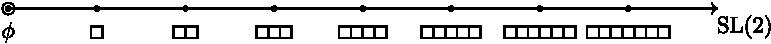
\includegraphics[]{images/sl2.pdf}
\end{center}

Within these, we have a subcategory of represenations of PGL(2):
\begin{center}
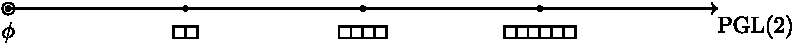
\includegraphics[]{images/pgl2.pdf}
\end{center}

The irreducible represenations of GL(2) look like this:
\begin{center}
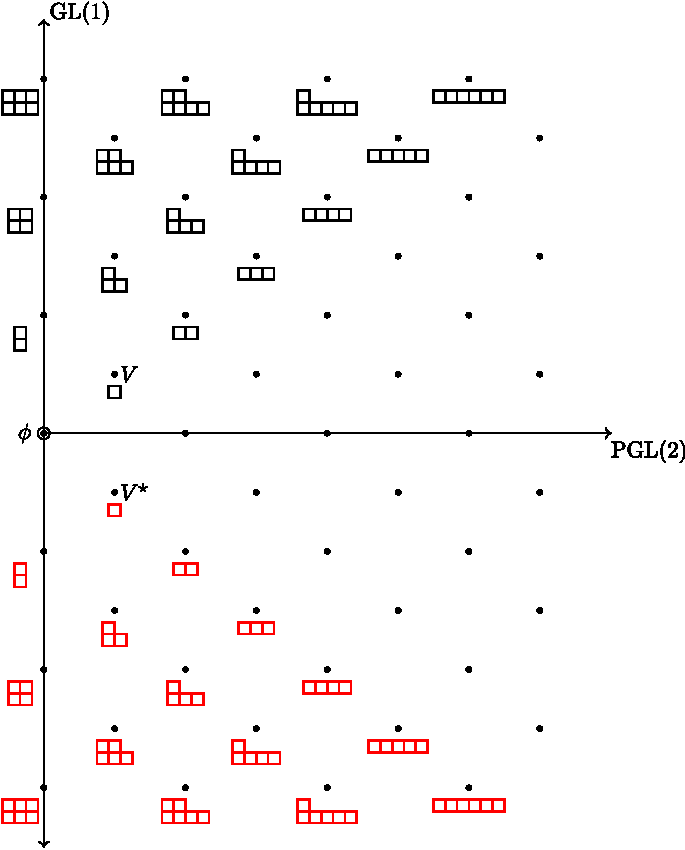
\includegraphics[scale=0.8]{images/gl2.pdf}
\end{center}
Where we have labelled the tautological (natural) represenation as $V$
and its dual as $V^{\star}.$

\section*{GL(3)}

\[
\begin{tikzcd}
    &  
    \SL(3) \arrow[rightarrowtail]{d}\arrow[two heads]{dr}{\mathrm{3-to-1}} &  \\
    \GL(1) \arrow[rightarrowtail]{r}{\mathrm{diag}} 
           \arrow[two heads]{dr}[below,left]{\mathrm{3-to-1\ }}  &  
    \GL(3) \arrow[two heads]{r}\arrow[two heads]{d}{\mathrm{det}}  &  \PGL(3)     \\
    &  \GL(1)             &     \\
\end{tikzcd}
\]

We start with a picture of the $\SL(3)$ kaleidoscope:
\begin{center}
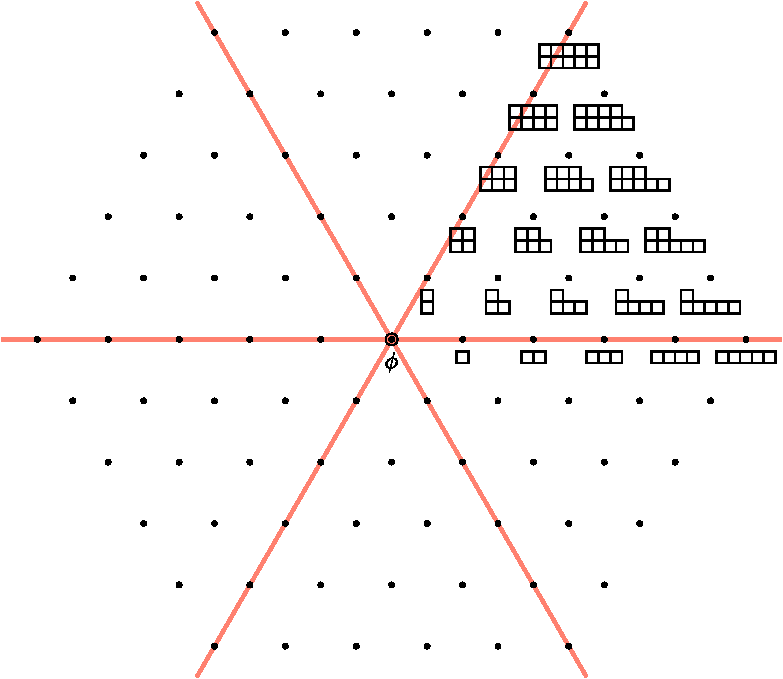
\includegraphics[scale=0.8]{images/sl3.pdf}
\end{center}

The epimorphism SL(3)$\to$PGL(3) is a 3-to-1 map,
and so we find the irreps of PGL(3) as an index 3 
sublattice of the SL(3) kaleidoscope:
\begin{center}
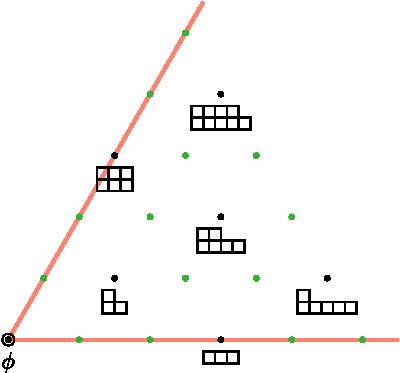
\includegraphics[scale=0.8]{images/pgl3.pdf}
\end{center}

The positive levels of $\GL(3)$:
\begin{center}
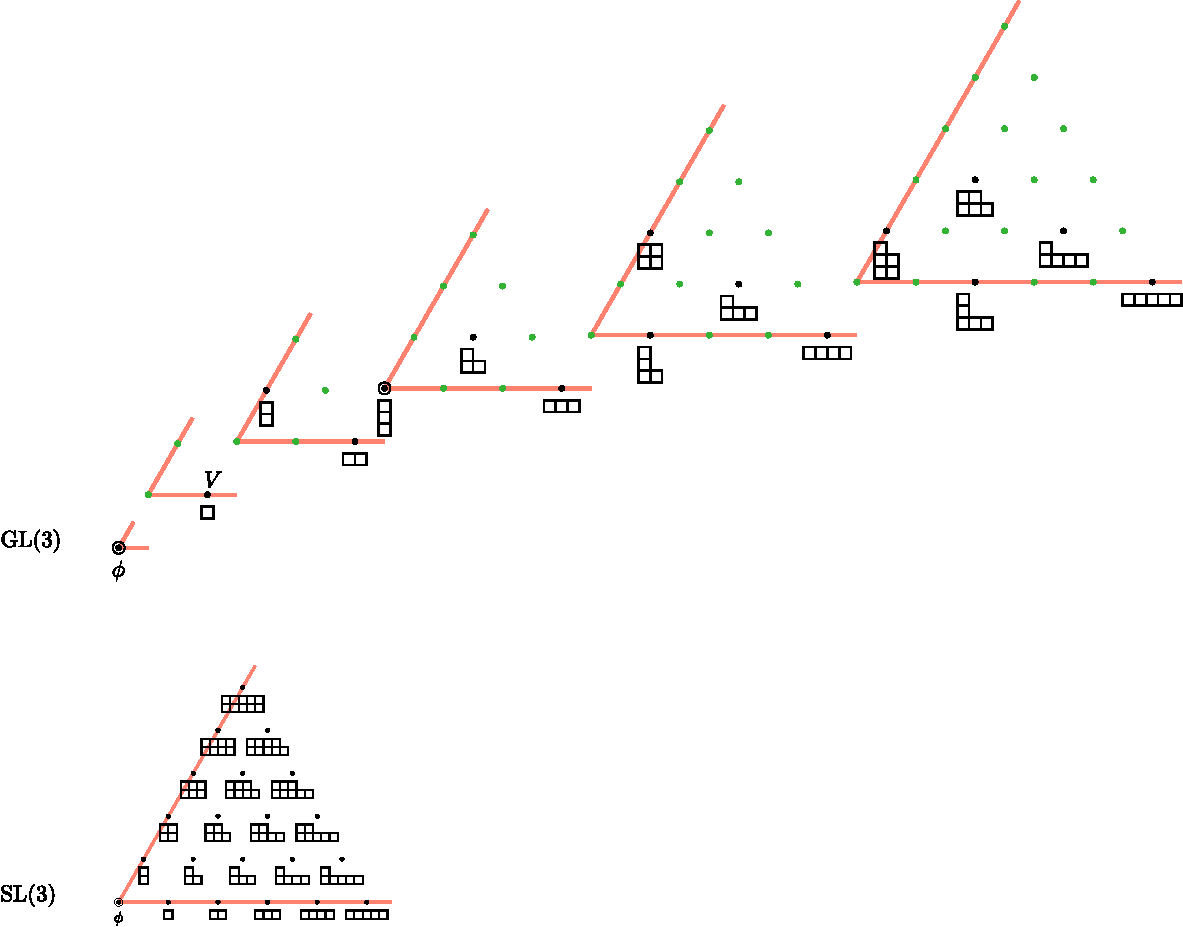
\includegraphics[scale=0.6]{images/gl3.pdf}
\end{center}

%\bibliography{refs2}{}
%\bibliographystyle{abbrv}

\end{document}
